%
% grundlagen.tex -- Paper zum Thema Optische Fouriertransformation <opt>
%
% (c) 2023 Marco Niederberger, Yanick Schoch; OST Ostschweizer Fachhochschule
%
% !TEX root = ../../buch.tex
% !TEX encoding = UTF-8
%
\section{Grundlagen\label{opt:section:grundlagen}}
\rhead{Von der Beugung zu Fourier}

\begin{figure}
    \centering
    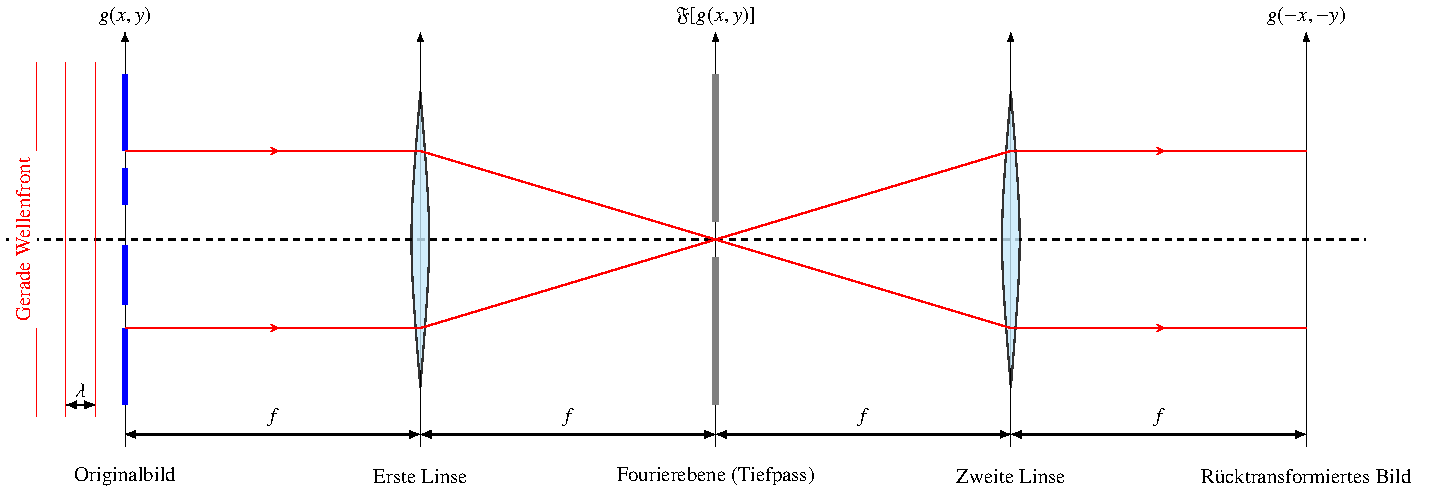
\includegraphics[width=\textwidth]{papers/opt/images/4fAufbau.pdf}
    \caption{Der 4f Aufbau ermöglicht eine Fouriertransformation des Originalbildes sowie eine Rücktransformation aus der Fourierebene.
    In dieser Abbildung wird die transformierte Funktion mit einem Tiefpass gefiltert.
    Weitere Details zu den Filtern folgen im Kapitel \ref{opt:section:filter}.}
    \label{opt:fig:4fAufbau}
\end{figure}

\subsection{Grundlagen Wellentheorie}
Beugung kurz erklärt

\subsubsection{Fressnel / Frauhofner}
Was ist der Unterschied zwischen den beiden Approximationen?

\subsection{Herleitung Fraunhofer Beugung}
In dieser Herleitung wird darauf eingegangen, wie die Fouriertransformierte mit Hilfe der Fraunhofer Beugung erhalten werden kann.

Betrachten wir zuerst, wie in TODO gezeigt, eine unendlich dünne linienförmige Lichtquelle, welche sich axial in beide Richtungen unendlich weit erstreckt.
Verallgemeinert kann es sich bei dieser Art von Quelle um eine beliebige elektromagentische Quelle handeln.
Somit kann durch anwenden der ersten Maxwellschen Gleichung
\begin{equation}
\oint_{S=\partial V} \varepsilon\vec{E} \cdot\, d\vec{S}
=
\int_{V}\rho\, dV
\end{equation}
die elektrische Feldstärke $\vec{E}$ an jedem beliebigen Punkt in Abhängigkeit des radialen Abstandes $r$ berechnet werden.
Angewendet auf die gegebene Geometrie des Zylindermantels lässt sich diese Gleichung mittels $dS = r d\varphi dl$ als
\begin{align}
\int_{0}^{a}\int_{0}^{2\pi} \varepsilon E\cdot 1 \cdot r\, d\varphi dl
&=
Q
\\
2\pi ra\varepsilon E
&=
Q
\end{align}
schreiben.
Die Deckflächen können aufgrund der infiniten Länge des Zylinders vernachlässigt werden.
Zu beachten sei zudem, dass die normierten vektoriellen Grössen $\hat{E}$ und $\hat{S}$ parallel verlaufen und sich ihr Skalarprodukt dementsprechend zu 1 vereinfacht.
Nach der elektrischen Feldstärke umgeformt lautet die Gleichung
\begin{equation}
E(r)
=
\frac{Q}{2\pi\varepsilon a} \cdot \frac{1}{r}
=
C \cdot \frac{1}{r}
\label{opt:equation:E}
\end{equation}
, wobei der konstante Anteil als $C$ zusammengefasst wurde.

Angenommen eine planare elektromagentische Welle, siehe TODO, treffe nun auf eine Blende mit einer unendlich langen und $b$ breiten Öffnung.
Ganz allgemein lässt sich jede Welle als
\begin{equation}
\zeta(x, t)
=
\zeta_0 \cdot e^{j(\omega t - \vec{k}\cdot\vec{x})}
\label{opt:equation:wave}
\end{equation}
ausdrücken.
Wie aus dem Physik Unterricht bereits bekannt ist, wird diese Welle am Spalt gebogen und sich hinter der Blende in Abhängigkeit von $b$ mehr oder weniger kreisförmig ausbreitet.
Zurückzuführen ist dieses Verhalten auf das Prinzip von Huygens TODO.
Dieses Verhalten der kreisförmigen Ausbreitung kann mittels der zuvor betrachteten Linienquellen modelliert werden.
Infinit viele dieser Linienquellen seien nun nebeneinander entlang der Öffnungsbreite $b$ angereiht.
Die Auswirkung dieser Quellen kann nun an jedem beliebigen Punkt hinter der Blende durch superponierung der einzelenen Quelleneinflüsse berechnet werden.

Ein Schirm werde nun im Abstand $l$ hinter der Blende angebracht, an welchem die elektrische Feldstärke auf verschiedenen Höhen $y_p$ gemessen werden soll.
Siehe TODO. Aus der geometrischen Anordnung geht hervor, dass
\begin{equation}
r
=
\sqrt{l^2 + (y_p-y)^2}
=
l \sqrt{1 + \frac{(y_p-y)^2}{l^2}}
\label{opt:equation:distance_r}
\end{equation}
beträgt.
Wie sich in Gleichung~\ref{opt:equation:integral_basic} zeigen wird, ist dieser Ausdruck aber noch nicht fundamental genug um eine analytische Lösung zu erhalten.
Durch anwenden der Binominalexpansion
\begin{equation}
(1 + \varepsilon)^n
\approx
1 + n\varepsilon
\end{equation}
, unter der Voraussetzung dass $\varepsilon \ll 1$ gilt, ist es möglich den Wurzelausdruck noch weiter zu vereinfachen.
Durch die geometrische Anordnung ist
\begin{equation}
(y_p-y)^2
\ll
l^2
\end{equation}
garantiert.
Somit kann die Bedingung
\begin{equation}
\varepsilon
=
\frac{(y_p-y)^2}{l^2}
\ll
1
\label{opt:equation:condition_epsilon}
\end{equation}
eingehalten werden.
Gleichung~\ref{opt:equation:distance_r} vereinfacht sich demnach näherungsweise zu
\begin{equation}
r
=
l \sqrt{1 + \frac{(y_p-y)^2}{l^2}}
\approx
l \left(1 - \frac{(y_p-y)^2}{2l^2}\right)
=
l - \frac{(y_p-y)^2}{2l}
.
\label{opt:equation:distance_r_simplified}
\end{equation}

All diese kleinen Einflüsse $dE$ der Linienquellen mit Breite $dy$ superponieren sich, wie bereits erwähnt, zur gesamten elektrischen Feldstärke am Auswertungspunkt.
Ein solcher Einfluss lässt sich nun mittels der Gleichungen~\ref{opt:equation:E} und \ref{opt:equation:wave} als
\begin{equation}
dE
=
E(r) \cdot \zeta(r, t) \cdot dy
=
\frac{C}{r} \cdot \zeta_0 \cdot e^{j(\omega t - \vec{k}\cdot\vec{r})} \cdot dy
\end{equation}
beschreiben.
Werden die Einflüsse der Linienquellen über den Spalt aufintegriert ergibt sich
\begin{equation}
E(y_p, t)
=
\int_{y_b}^{y_b+b}\frac{C\zeta_0}{r} \cdot e^{j(\omega t - \vec{k}\cdot\vec{r})} \,dy
.
\label{opt:equation:integral_basic}
\end{equation}
Durch ausklammern von Konstanten und einsetzen der Gleichung~\ref{opt:equation:distance_r_simplified} vereinfacht sich das Integral weiter zu
\begin{align}
E(y_p, t)
&=
C\zeta_0 \cdot e^{j\omega t} \cdot \int_{y_b}^{y_b+b} \frac{e^{-j\vec{k}\cdot\vec{r}}}{r} \,dy
\\
&=
C\zeta_0 \cdot e^{j\omega t} \cdot \int_{y_b}^{y_b+b} \frac{e^{-jkr \cdot 1}}{r} \,dy
\\
&=
C\zeta_0 \cdot e^{j\omega t} \cdot \int_{y_b}^{y_b+b} \frac{e^{-jdl} \cdot e^{-jk\frac{(y_p-y)^2}{2l}}}{l - \frac{(y_p-y)^2}{2l}} \,dy
\\
&=
C\zeta_0 \cdot e^{j\omega t} \cdot e^{-jdl} \cdot \int_{y_b}^{y_b+b}\frac{e^{-jk\frac{(y_p-y)^2}{2l}}}{l - \frac{(y_p-y)^2}{2l}} \,dy
.
\end{align}
Wiederum konnte das Skalarprodukt der normierten Grössen $\hat{k}$ und $\hat{r}$ aufgrund Parallelität als 1 gekürtzt geschrieben werden.
Desweiteren kann der Ausdruck im Nenner des Integrals als $l$ vereinfacht werden.
Dies ist nur zulässig aufgrung von Gleichung~\ref{opt:equation:condition_epsilon}.
Dasselbe darf jedoch nicht auf den Nenner dieses Bruches angewandt werden.
Im Falle von rotem Licht, dessen Wellenlänge $\lambda$ rund 700nm beträgt TODO
